\documentclass[12pt]{article}

\usepackage[a4paper, margin=1in]{geometry}
\usepackage{setspace}
\usepackage{graphicx}
\usepackage{booktabs}
\usepackage{amsmath}
\usepackage{float}
\usepackage{enumitem}
\usepackage[numbers]{natbib}
\usepackage{xcolor}
\usepackage{titlesec}
\usepackage{fancyhdr}
\usepackage{titling}
\usepackage{tocloft}
\usepackage{hyperref}

\graphicspath{{./images/}}
\usepackage{subcaption}

\hypersetup{
    colorlinks=true,
    linkcolor=blue,
    citecolor=blue,
    urlcolor=blue
}

\setstretch{1.15}

% ============================================================
% COLORS
% ============================================================

\definecolor{darkblue}{RGB}{0,51,102}
\definecolor{lightgray}{RGB}{240,240,240}

% ============================================================
% SECTION FORMATTING
% ============================================================

\titleformat{\section}
{\large\bfseries}
{\thesection.}{0.5em}{}

\titleformat{\subsection}
{\normalsize\bfseries}
{\thesubsection}{0.5em}{}

% ============================================================
% HEADER / FOOTER
% ============================================================

\pagestyle{fancy}
\fancyhf{}
\fancyhead[L]{Credit Portfolio Risk Analysis}
\fancyhead[R]{\thepage}
\renewcommand{\headrulewidth}{0.4pt}

% ============================================================
% TABLE OF CONTENTS STYLE
% ============================================================

\renewcommand{\cftsecleader}{\cftdotfill{\cftdotsep}}

% ============================================================
% TITLE PAGE
% ============================================================

\title{
    \vspace{4cm}
    {\Huge \bfseries Credit Portfolio Risk Analysis} \\
    \vspace{1.5cm}
    {\Large Final Assignment Report} \\
    \vspace{2cm}
}

\author{
    \Large Student Name \\
    \vspace{0.5cm}
    Course Name \\
    Instructor Name
}

\date{\today}

% ============================================================
% DOCUMENT
% ============================================================

\begin{document}

% ============================================================
% TITLE PAGE
% ============================================================

\begin{titlepage}
    \centering

    \vspace*{2cm}

    {\Huge \bfseries \textbf{Theoretical and Empirical Applications of Single-Factor, Multi-Factor, and Beta-Binomial Models}

 \par}





    \vspace{2cm}

    \rule{0.8\textwidth}{0.5pt}
    \rule{0.8\textwidth}{0.5pt}

    \vspace{3cm}

    \begin{center}
    \large
    \textbf{Student:} Jialin Geng \\
    \vspace{0.3cm}
    \textbf{Portfolios:} Portfolio 1, 2 and 3 \\
    \vspace{0.3cm}
    \textbf{Course:} Introduction to Credit Risk and Applications in Python  \\
    \vspace{0.3cm}
    \textbf{Date:} \today
    \end{center}

    \vspace{3cm}

    \rule{0.8\textwidth}{0.5pt}
    \rule{0.8\textwidth}{0.5pt}




\end{titlepage}

% ============================================================
% TABLE OF CONTENTS
% ============================================================

\newpage

\tableofcontents

\newpage

% ============================================================
% INTRODUCTION
% ============================================================

\section{Introduction}
In credit risk management and quantitative investing, assessing default correlation and the potential loss distribution of a portfolio is of paramount importance. Traditional credit asset pricing and economic capital measurement typically rely on latent variable models.

This report aims to conduct systematic credit risk modeling for a specific asset portfolio by utilizing the provided 20-year historical default data, as well as individual stock and industry index return data. The report focuses on three mainstream credit risk measurement models:

\begin{itemize}
\item \textbf{Single-Factor Model}: Based on the Vasicek framework, it assumes that all entities are jointly exposed to a single macroeconomic factor.


\item \textbf{Multi-Factor Model}: It introduces industry and regional factors to capture systemic risk sources at a more granular level.


\item \textbf{Beta-Binomial Model}: By treating the probability of default (PD) as a random variable following a Beta distribution, it directly characterizes default clustering and excess variance within a mixed binomial distribution framework.


\end{itemize}
This report will systematically elaborate on the theoretical frameworks of the aforementioned models, perform parameter estimation by combining historical asset returns and default data, and compare the strengths and weaknesses of each model in describing the potential default distribution of the portfolio.




% ============================================================
% DATA
% ============================================================

\section{Data}
The dataset utilized in this study encompasses multiple dimensions, including credit portfolios, corporate fundamental information, historical default records, and high-frequency capital market returns. Its specific composition is as follows:

\begin{itemize}
\item \textbf{Portfolio Data (Portfolio 1, 2, 3)}: This includes the Exposure at Default (EAD), Loss Given Default (LGD), and individual Probability of Default (PD) for underlying assets across different industries. Among them, Portfolio 1 is primarily concentrated in Industry A, Portfolio 2 is primarily concentrated in Industry B, and Portfolio 3 is a cross-industry mixed asset portfolio.


\item \textbf{Corporate Entity Information (Entities Info)}: This contains the codes, names, industry classifications (Industry A/B), geographic regions (Europe, North America, Asia, etc.), benchmark PD indicators, and analyst rating notes for 103 companies.


\item \textbf{Historical Default Observation Data (Default History)}: This covers an annual observation time series over the past 20 years, recording whether each entity experienced a default event (default\_event=1.0 or 0.0) in each respective year.


\item \textbf{Market Return Data}: This includes the daily stock returns for each enterprise as well as the corresponding industry index returns, providing an empirical capital market basis for estimating factor model sensitivities (Beta) and asset correlations.


\end{itemize}




% ============================================================
% METHODOLOGY
% ============================================================

\section{Methodology}

\subsection{Single-Factor Model}
The single-factor model is primarily based on the Vasicek model, which extends from the Merton structural model framework. This model assumes that the latent critical variable $Xi$ driving the change in the asset value of borrower i is determined solely by a common systemic macroeconomic factor $F$ and an idiosyncratic credit risk factor (i.e., unsystematic risk) $\epsilon_i$:

\[X_i = \rho F + \sqrt{1 - \rho^2} \epsilon_i\]

\subsection{Multi-Factor Model}
While the single-factor model is elegant and analytically tractable, its assumption that all enterprises are driven by the same economic factor overlooks structural differences such as industry and geography. To more accurately characterize complex asset correlations, multi-factor models (such as the CreditMetrics framework) extend the critical variable to be driven by a vector of systemic factors:
\[X_i = \beta_{i,1} F_1 + \beta_{i,2} F_2 + \dots + \beta_{i,k} F_k + \eta_i \epsilon_i\]

Where $F = [F_1, F_2, \dots, F_k]'$ represents the vector of systemic factors composed of different industry returns or regional macroeconomic indicators, which may themselves exhibit normal correlation. $\beta_i$ is the vector of the borrower's sensitivities to each factor. To maintain the standard normal distribution property of $X_i$, the coefficient of the residual term must satisfy $\eta_i = \sqrt{1 - \sum_{j=1}^{k} \beta_{i,j}^2}$. The correlation between any two enterprises will be directly determined by their common factor exposures and the covariance matrix of the factors themselves: $\text{Corr}(X_i, X_j) = \beta_i^\prime \Sigma_F \beta_j$.

\subsection{Beta-Binomial Model}
The Beta-Binomial model is a mixture model that does not rely directly on the structural mapping of asset values, but rather starts directly from the probability distribution of default rates. It assumes that in a portfolio containing $N$ homogeneous borrowers, the default probability $P$ of each firm is a random variable that follows a Beta distribution: $P \sim \text{Beta}(\alpha, \beta)$.

When the macroeconomic environment is fixed (i.e., $P$=$p$), the conditional probability of $k$ default events occurring in the portfolio follows a binomial distribution. By integrating over the marginal distribution of $P$, the unconditional overall probability distribution of the number of defaults can be obtained:
\[P(K=k) = \binom{N}{k} \frac{B(\alpha + k, \beta + N - k)}{B(\alpha, \beta)}\]
Using the Method of Moments (MoM), the key parameters of the model can be derived back from the mean $\mu_p$   and variance $\sigma_p^2$ of historical default rates:
\[\alpha = \mu_p \left[ \frac{\mu_p (1 - \mu_p)}{\sigma_p^2} - 1 \right] , \beta = (1 - \mu_p) \left[ \frac{\mu_p (1 - \mu_p)}{\sigma_p^2} - 1 \right]\]
The implied default correlation corresponding to this model can be expressed as:
\[\rho_D = \frac{1}{\alpha + \beta + 1}\]


% ============================================================
% RESULTS
% ============================================================

\section{Results and Discussion}

\subsection{Factor Model}

\subsubsection{Single-Factor Model}
Modeling was conducted separately for the three portfolios, and the results are summarized in Figure \ref{fig:multi_factor_comparison}. From these findings, we can observe that the Value at Risk (VaR) of Portfolio 3 is significantly higher than that of Portfolio 1 and Portfolio 2. Different industrial sectors are interconnected; if correlations exist within the same systemic factor (Industry), a default triggered by this factor can lead to far more severe default losses (VaR) than under normal conditions. Therefore, for this type of portfolio, institutions must set aside more Economic Capital (EC) to absorb potential Unexpected Losses (UL) that may be incurred over the horizon of the following year. Observing Table \ref{tab:portfolio_var_factor_model}, we can also find that the VaR calculated by the analytical method is lower than that calculated by the simulation method.
\begin{figure}[H]
    \centering  % <--- 这一行是关键，它会使环境内的内容水平居中
    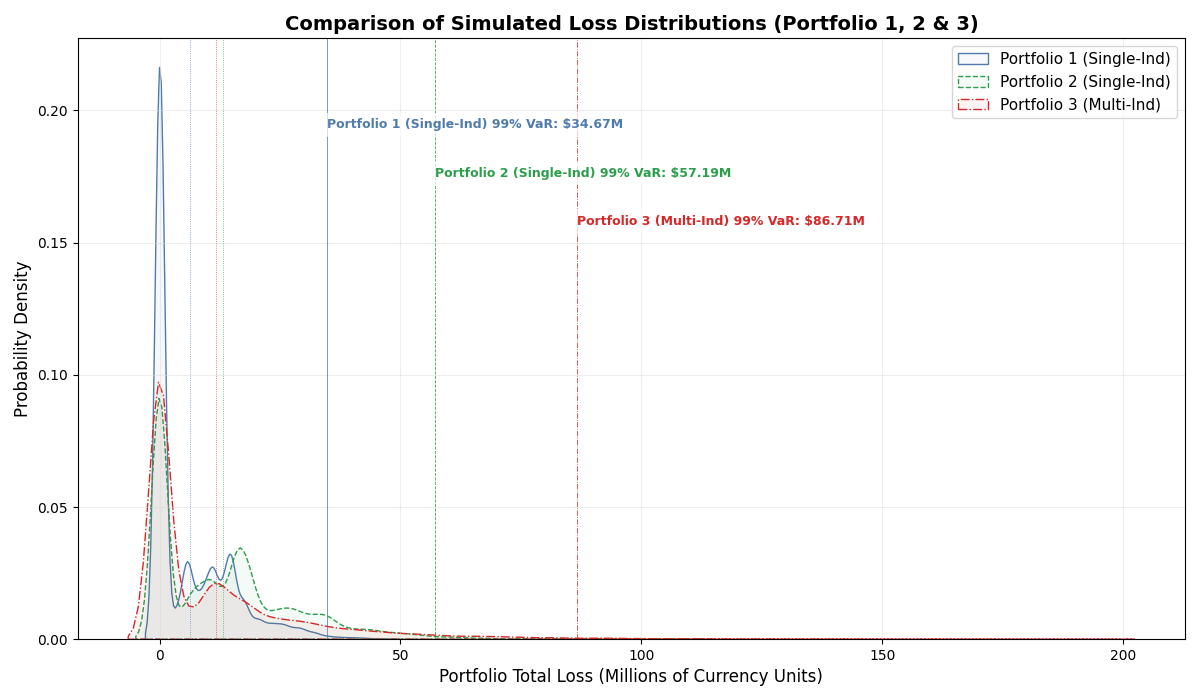
\includegraphics[width = 0.5\textwidth]{figure_1}
    \caption{Comparison of Simulated Loss Distribution (Portfolio 1, 2 and 3)}
    \label{fig:one_factor_comparison}
\end{figure}

\begin{table}[H]
    \centering
    \caption{Portfolio VaR(99\%) Comparison}
    \label{tab:portfolio_var_factor_model}
    \begin{tabular}{|l|p{4.2cm}|p{3.8cm}|p{4.2cm}|}
        \hline
        \textbf{Portfolio} & \textbf{One-Factor Monte Carlo (VaR 99\%)} & \textbf{Vasicek Analytical (VaR 99\%)} & \textbf{Multi-Factor Monte Carlo (VaR 99\%)} \\
        \hline
        \hline
        \textbf{Portfolio 1} & \$34.67M & \$12.00M & \$52.35M \\
        \hline
        \textbf{Portfolio 2} & \$57.19M & \$27.94M & \$110.06M \\
        \hline
        \textbf{Portfolio 3} & \$86.71M & N/A (Single-Factor Only) & \$83.25M \\
        \hline
    \end{tabular}
\end{table}


\subsubsection{Multi-Factor Model}
As illustrated in Figure \ref{fig:multi_factor_comparison}, under the multi-factor model framework, the inclusion of additional systemic factors amplifies the fat-tail effect, thereby increasing the Value at Risk (VaR). Furthermore, as shown in Figure \ref{fig:multi_factor_comparison}-(c), the VaR simulated by the multi-factor model is higher than that from the single-factor model, which is more aligned with reality. Under the influence of multiple factors, the fat-tail effect can be further exacerbated, leading to an even higher VaR. Consequently, financial institutions need to set aside more Economic Capital (EC) to absorb potential Unexpected Losses (UL) that may be incurred over the horizon of the following year.

Observing Table \ref{tab:portfolio_var_factor_model}, however, if interdependencies exist among identical systemic factors within the portfolio (as observed in Portfolio 3), the variance in VaR values under the multi-factor model becomes less pronounced. This is because when simulating Portfolio 3—which comprises two distinct industrial factors (Industry A and Industry B)—the model inherently accounts for the impacts of different factors on the latent variables, essentially functioning as a multi-factor model. As a result, the difference in VaR at this point is not particularly significant.

\begin{figure}[H]
    \centering
    % 第一张图 (Portfolio 1)
    \begin{subfigure}{0.31\textwidth}
        \centering
        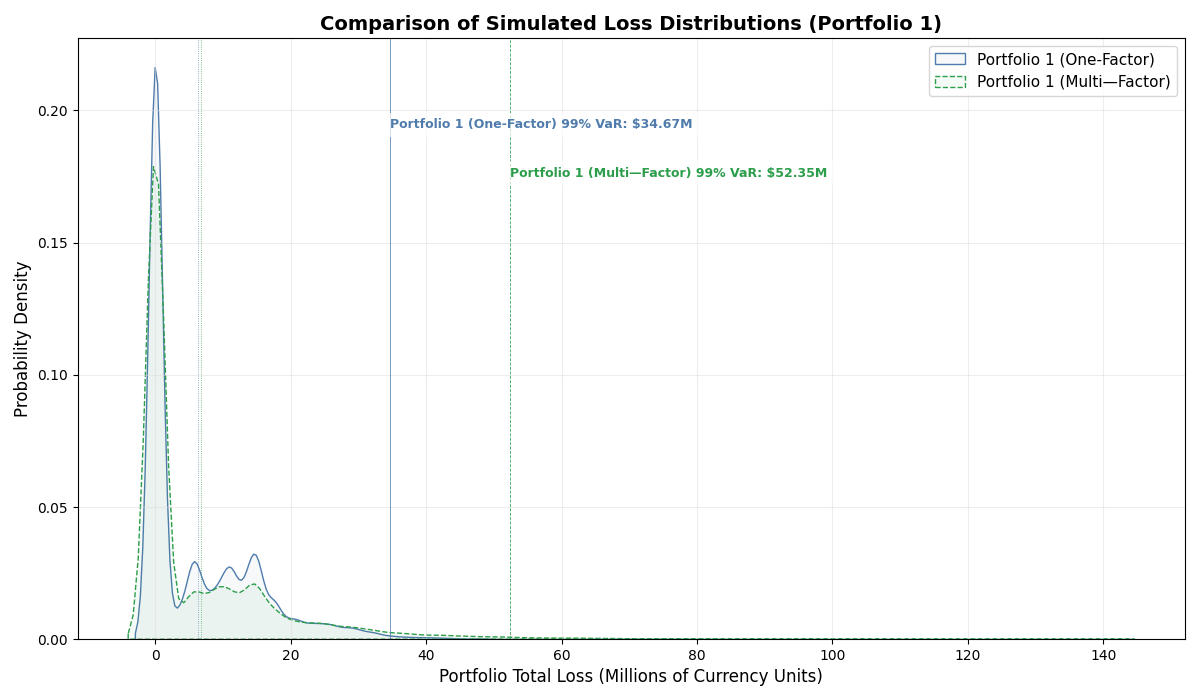
\includegraphics[width=\textwidth]{figure_2a}
        \caption{portfolio 1}
    \end{subfigure}
    \hfill
    % 第二张图 (Portfolio 2)
    \begin{subfigure}{0.31\textwidth}
        \centering
        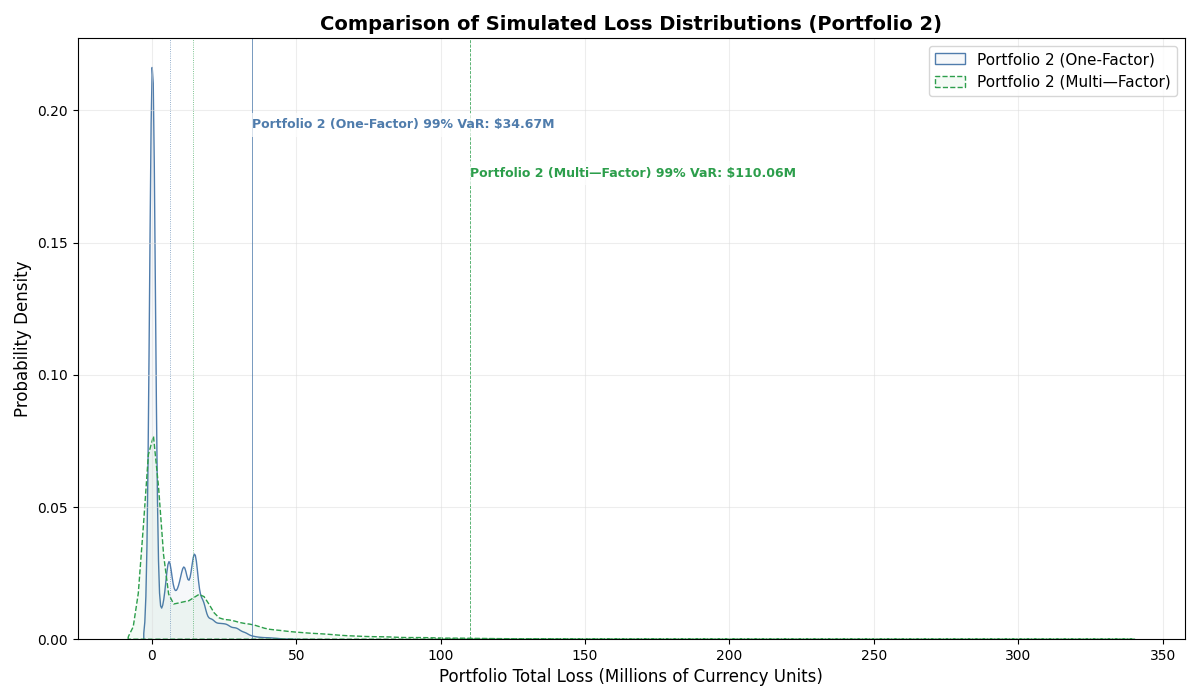
\includegraphics[width=\textwidth]{figure_2b}
        \caption{portfolio 2}
    \end{subfigure}
    \hfill
    % 第三张图 (Portfolio 3)
    \begin{subfigure}{0.31\textwidth}
        \centering
        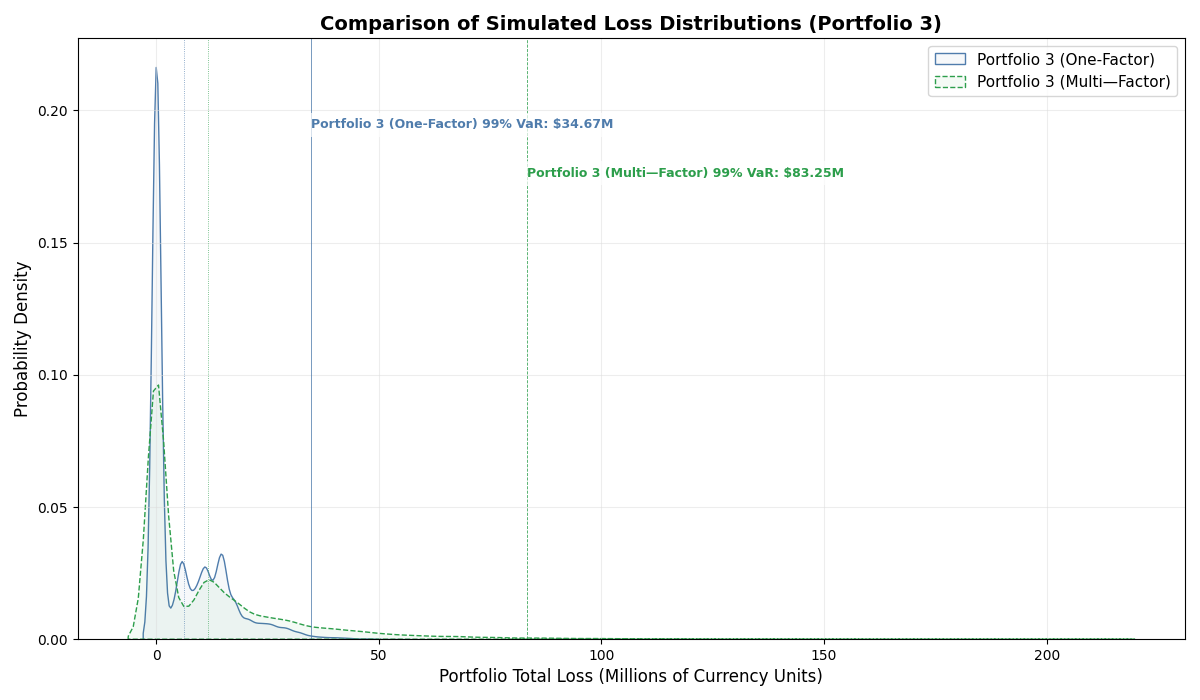
\includegraphics[width=\textwidth]{figure_2c}
        \caption{portfolio 3}
    \end{subfigure}

    \vspace{0.5cm} % 稍微留出点空隙
    \caption{Comparison of Simulated Loss Distribution for Portfolio 1, 2, and 3 with Multi-Factor Model}
    \label{fig:multi_factor_comparison}
\end{figure}


\subsection{Beta-Binomial Model}
The Beta-Binomial model was utilized again to simulate Portfolios 1 and 2. As illustrated in Figure \ref{fig:simulation under beta_binomial model}, this further verifies that the default loss does not follow a normal distribution; instead, more extreme values occur, manifesting as a so-called "fatter tail."

As an additional attempt, the code was obtained after consulting the AI (named Simulation for Portfolio 3 under Beta-Binomial Model.py).

\begin{figure}[H]
    \centering
    \begin{subfigure}{0.48\textwidth}
        \centering
        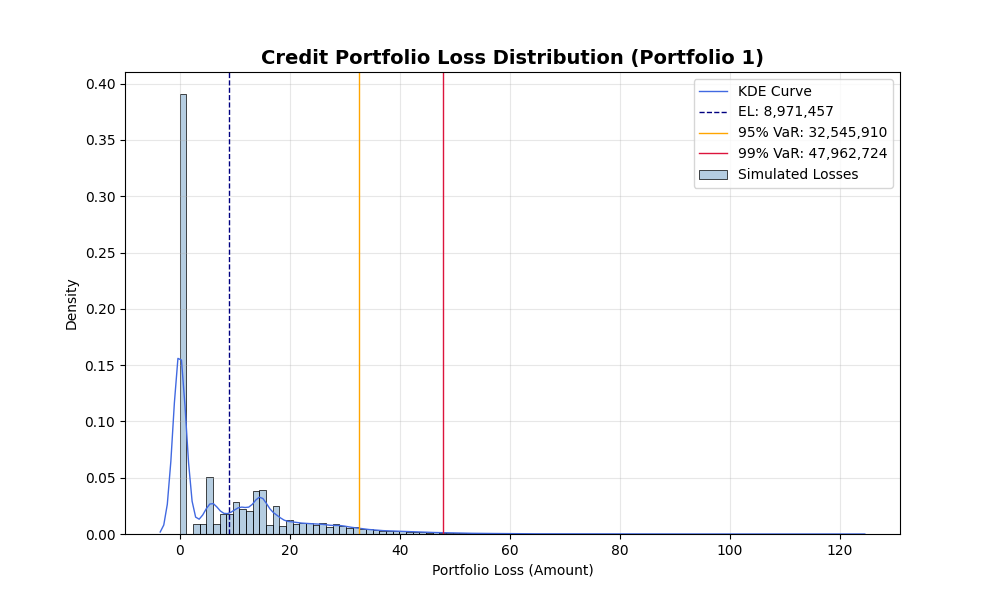
\includegraphics[width=\textwidth]{figure_3a}
        \caption{portfolio 1}
    \end{subfigure}
    \hfill
    \begin{subfigure}{0.48\textwidth}
        \centering
        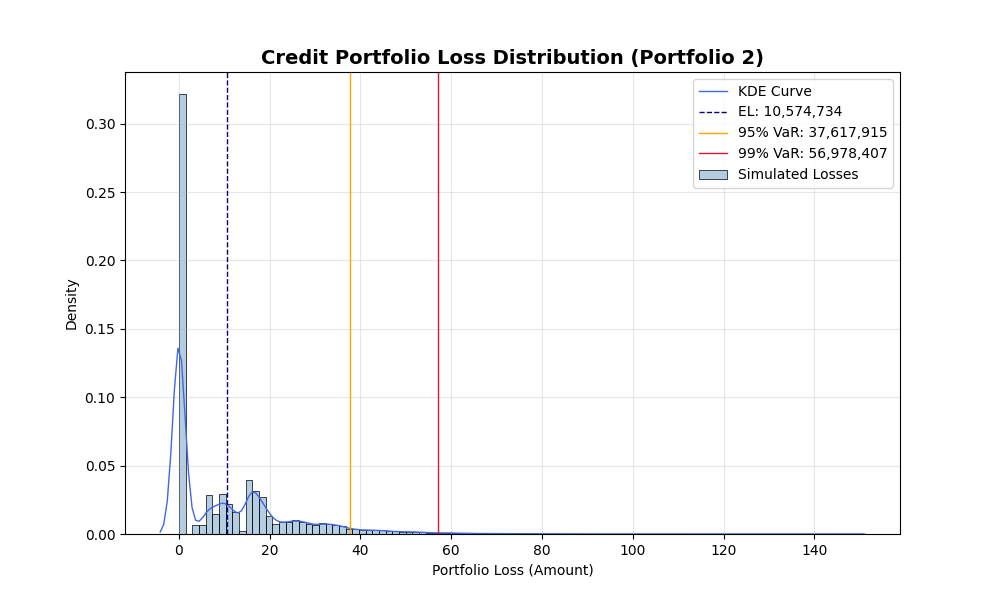
\includegraphics[width=\textwidth]{figure_3b}
        \caption{portfolio 2}
    \end{subfigure}
    \caption{Credit Portfolio Loss Distribution under Beta-Binomial Model}
    \label{fig:simulation under beta_binomial model}
\end{figure}



% ============================================================
% CONCLUSION
% ============================================================

\section{Conclusion}
The probabilities of correlated defaults will have a fatter tail, indicating a higher likelihood of extreme losses. Although the Beta-Binomial model has traditionally been restricted to a single-factor environment, future research could explore potential methodologies to implement this model within a multi-factor framework, thereby further validating the aforementioned conclusions.



% ============================================================
% REFERENCES
% ============================================================

\newpage

\bibliographystyle{apalike}

\begin{thebibliography}{}

\bibitem{key1}
    Lütkebohmert-Holtz, E., \& Shen, H. (2026). \textit{Introduction to Credit Risk and Applications in Python}. University of Freiburg Lecture Material.

\bibitem{key2}
    Vasicek, O. A. (2002). \textit{The distribution of loan portfolio value}. Risk, 15(12), 160-162.

\bibitem{key3}
    Gupton, G. M., Finger, C. C., \& Bhatia, M. (1997). \textit{CreditMetrics—Technical Document}. J.P. Morgan, New York.


\end{thebibliography}

\end{document}
```
